\chapter{Activity V1}

\section{Sample Input File}
\label{section:sampleinputfileactivity1}


\begin{lstlisting}[style=sOutputFile,caption={Activity V1 Input File}]
#elements
Fe 100
#isotopes
"/home/ben/activity/data/isotopes.txt"
#decaymodes
"/home/ben/activity/data/decaymodes.txt"
#gammaenergies
"/home/ben/activity/data/gammaenergies.txt"
#xsfiles
"/home/ben/activity/data/xs"
#trajfile
"Fe36MeV.exyz"
#polyfitorder
5
#integrationgranularity
10
#beamflux
0.5 uA
#beamenergy
36 MeV
#beamduration
300 s
#beamarea
100 mm2
#amtime
260000 s
#timestep
1000 s
#projectile
1 1
#targetthickness
0.5 mm
#materialdensity
8000 kgm3
#vpi
60.2
#individualisotopeactivity
yes
#verboseterminal
yes
#targetdpa
0.0
#gammachartresolution
200
\end{lstlisting}

\FloatBarrier





\section{Paper published in Computer Physics Communications}
\label{section:activityv1published}

The Activity code was published in the Computer Physics Communications journal and this is included in the following pages.  It was submitted in 2015 and published in 2017.

\clearpage

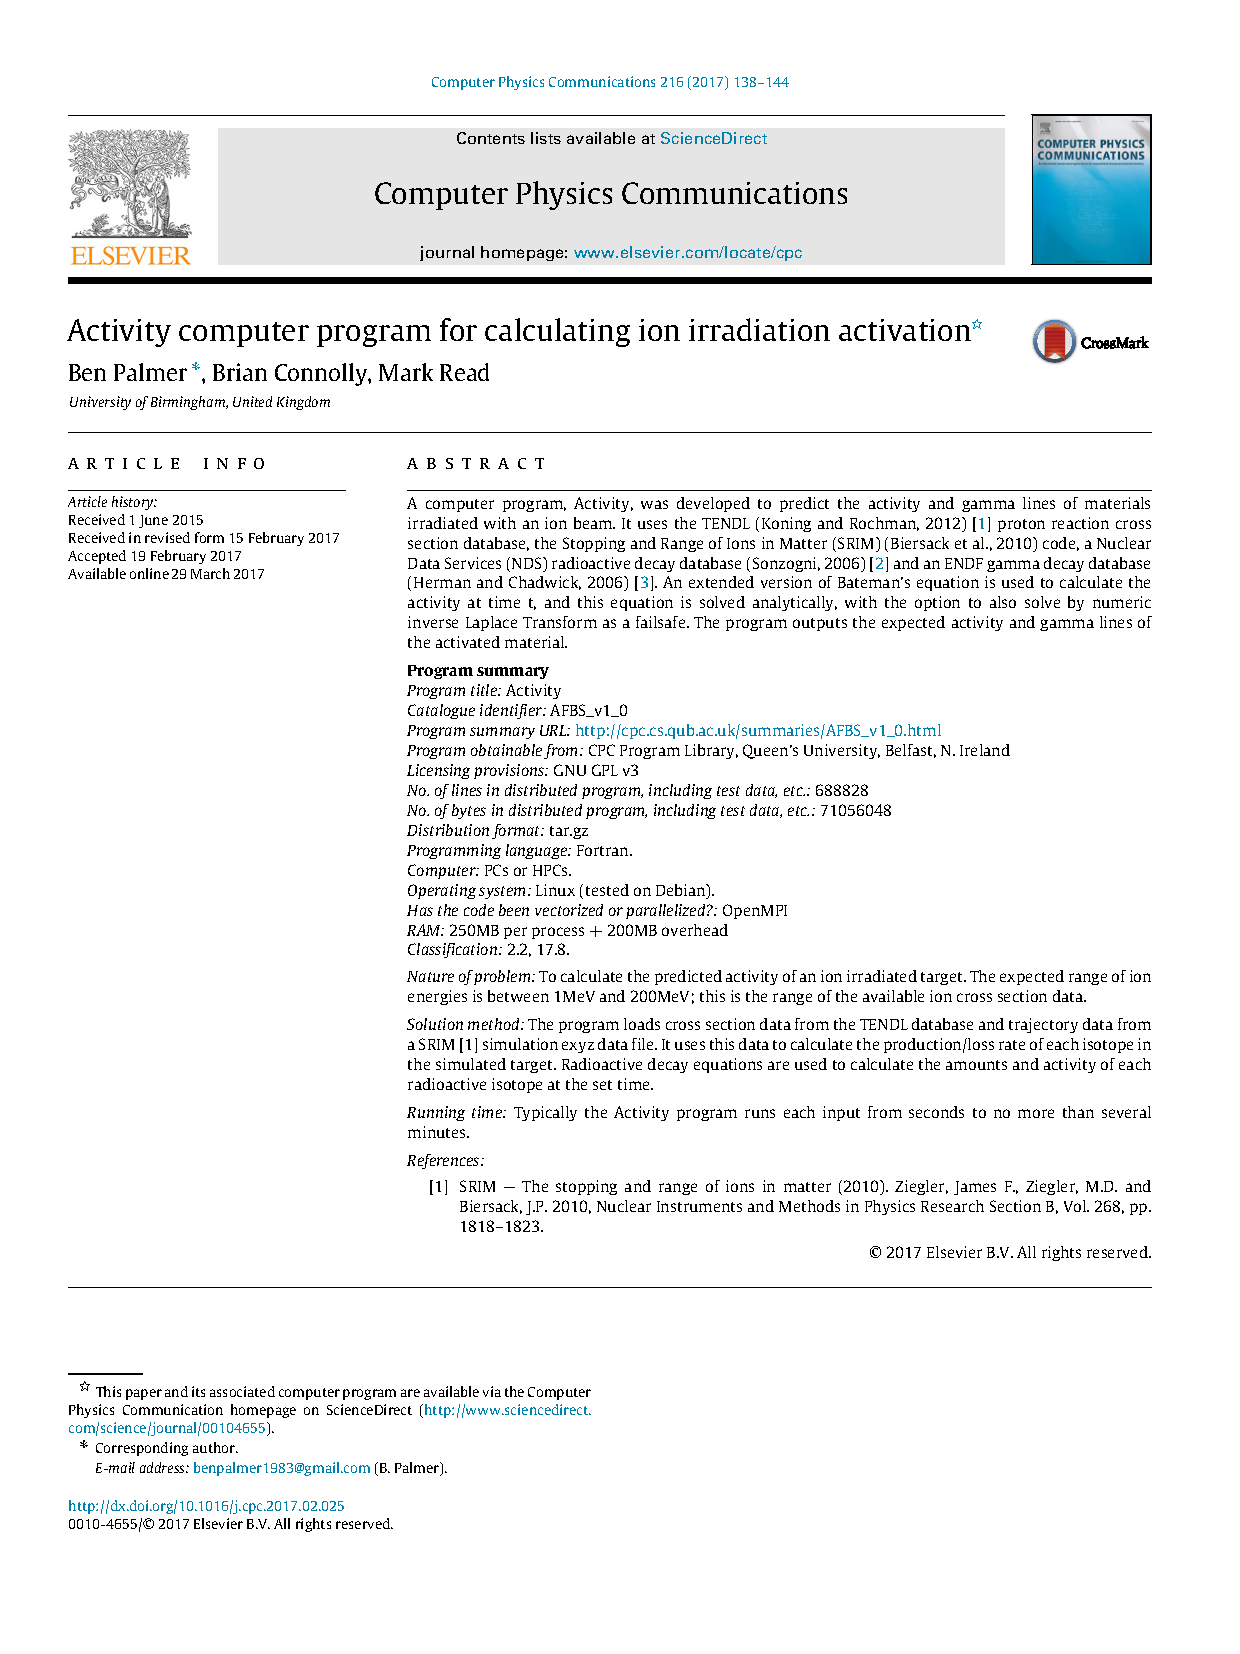
\includepdf[
    clip=0mm 0mm 0mm 0mm,
    trim=0mm 0mm 0mm 0mm,
    pages=-,
    frame,
    scale=.90,
    pagecommand={}]{appendix/activity_code/published.pdf}

\FloatBarrier

\section{Accompanying Manual}
\label{section:activityv1manual}

The accompanying manual for the Activity code is included in the following pages.

\clearpage


\includepdf[
    clip=0mm 0mm 0mm 0mm,
    trim=0mm 0mm 0mm 0mm,
    pages=-,
    frame,
    scale=.90,
    pagecommand={}]{appendix/activity_code/activity_v1_manual.pdf}










